\chapter{Lambda Architecture}
\label{chap:lambda_architecture}

The Lambda architecture \cite{MarzWarren201401} is a new solution
for creating a BigData system of any type. It provides the model for scalable, fault-tolerant, distibuted processing
of data. It uses both batch and online processing to answer the queries. It
provides human fault-tolerance, what is often overlooked in other approaches.
The Lambda architecture lets developer to concentrate on the bussiness-logik,
instead of thinking about distributing computations, replication of dataset and
how to manage intense grow of input data.

The core of the Lambda architecture is the equation "query = function(all
data)". The idea is that to answer any kind of query one can take the whole
dataset and execute particular function. The problem is that it is unreasonably
expensive, and even infeasible in most of cases. To solve this issue one can
create views, that are helpful for answeing particular queries, in advance. The
only problem of such approach is that indexing all the data and creating views
is high-latency operation. It can take several hours to be done. To overcome
this delay the Lambda architecture provides online processing of the data coming
in the real-time, that has not yet appeared in the precomputed views. As a
result, to answer the query both things are used: views, computed on the whole
dataset in advance, and sketch of the very new data.

One key aspect of the Lambda architecture, that makes a difference with the
other approaches, is that human fault-tolerance is concerned inherently. This is
important issue, because mistakes in programming code are guarantied. And as a
result, deleting or updating the data in a wrong way is also possible. The Lambda
architecture doesn't allow to modify data. This is called \mnote{Immutability}
immutability. Data can be only added, and never can be deleted or updated. This
leads to completely different model of storing data. Instead of having simple
tuple for a particular entity, every value of a tuple is stored separately and
has timestamp. Such technique allows to have the whole history of editions of
all attributes, what can be useful to make quesries that use history of changes.
At the same time the actual value is the one with the oldest timestamp.

\authorsection{General structure}{VI}

General view of the Lambda architecture is depicted on the
Figure~\ref{fig:lambda_architecture}.

\begin{figure}[H]
  \centering
  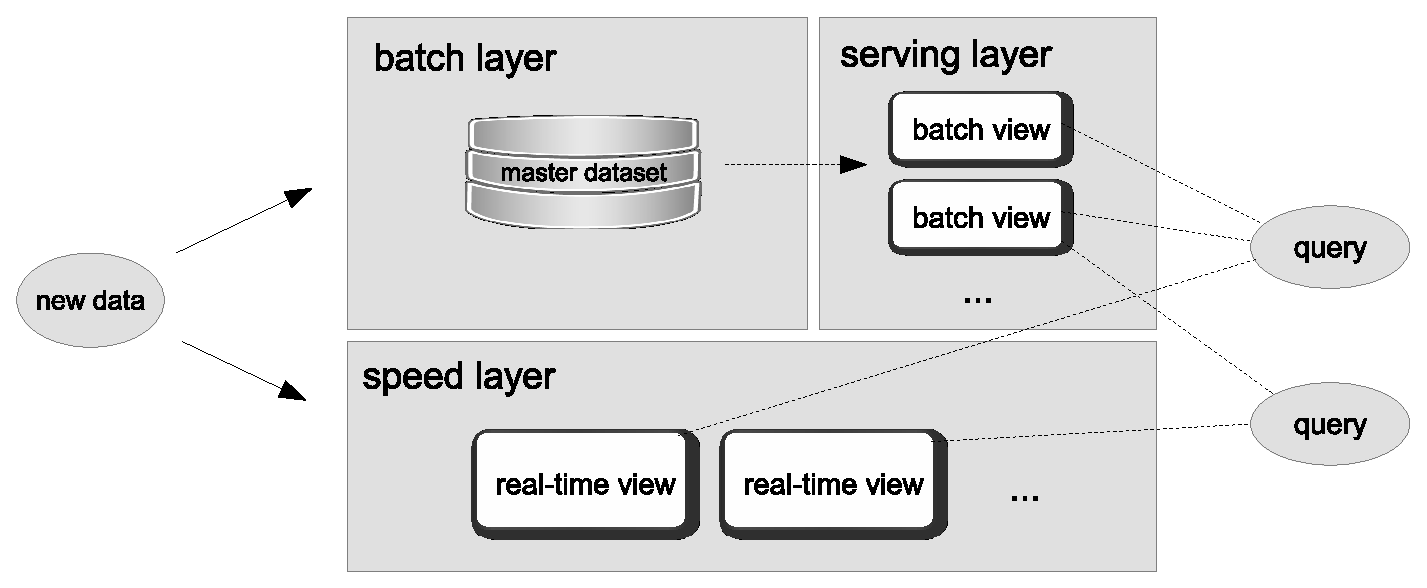
\includegraphics [width=0.9\textwidth]{images/LambdaArchitecture}
  \caption{General structure of the Lambda architecture}
  \label{fig:lambda_architecture}
\end{figure}


\authorsection{Interaction of the components}{VI}

\authorsection{Batch layer}{VI}

\authorsection{Serving layer}{VI}

\authorsection{Speed layer}{VI}